\documentclass{article}

\usepackage{amsmath}
\usepackage{multirow}
\usepackage{graphicx}
\usepackage{booktabs}

\title{ISOM3360 Assignment: ROC Curve}
\author{Zhang Yichen}

\begin{document}
\maketitle

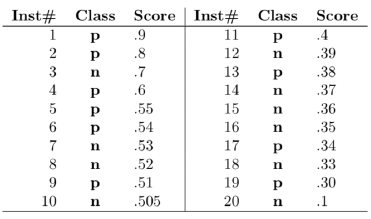
\includegraphics{Assignment}

\section{Answer}
\noindent By changing the decision threshold $x$, we can get different pairs of TPR/FPR.

\subsection*{$x \in (0.9, 1]$}

\begin{center}
    \begin{tabular}{@{}cc|cc@{}}
        \multicolumn{1}{c}{} &\multicolumn{1}{c}{} &\multicolumn{2}{c}{Predicted} \\ 
        \multicolumn{1}{c}{} & 
        \multicolumn{1}{c|}{} & 
        \multicolumn{1}{c}{p} & 
        \multicolumn{1}{c}{n} \\ 
        \cline{2-4}
        \multirow[c]{2}{*}{\rotatebox[origin=tr]{90}{Actual}}
        & p     & 0     & 10    \\[1.5ex]
        & n      & 0     & 10    \\ 
        \cline{2-4}
    \end{tabular}   
\end{center}

\begin{align*}
    TPR &= \frac{0}{0+10} = 0.0 \\
    FPR &= \frac{0}{0+10} = 0.0
\end{align*}

\subsection*{$x \in (0.8, 0.9]$}

\begin{center}
    \begin{tabular}{@{}cc|cc@{}}
        \multicolumn{1}{c}{} &\multicolumn{1}{c}{} &\multicolumn{2}{c}{Predicted} \\ 
        \multicolumn{1}{c}{} & 
        \multicolumn{1}{c|}{} & 
        \multicolumn{1}{c}{p} & 
        \multicolumn{1}{c}{n} \\ 
        \cline{2-4}
        \multirow[c]{2}{*}{\rotatebox[origin=tr]{90}{Actual}}
        & p     & 1     & 9    \\[1.5ex]
        & n      & 0     & 10    \\ 
        \cline{2-4}
    \end{tabular}   
\end{center}

\begin{align*}
    TPR &= \frac{1}{1+9} = 0.1 \\
    FPR &= \frac{0}{0+10} = 0.0
\end{align*}

\subsection*{$x \in (0.7, 0.8]$}

\begin{center}
    \begin{tabular}{@{}cc|cc@{}}
        \multicolumn{1}{c}{} &\multicolumn{1}{c}{} &\multicolumn{2}{c}{Predicted} \\ 
        \multicolumn{1}{c}{} & 
        \multicolumn{1}{c|}{} & 
        \multicolumn{1}{c}{p} & 
        \multicolumn{1}{c}{n} \\ 
        \cline{2-4}
        \multirow[c]{2}{*}{\rotatebox[origin=tr]{90}{Actual}}
        & p     & 2     & 8    \\[1.5ex]
        & n      & 0     & 10    \\ 
        \cline{2-4}
    \end{tabular}   
\end{center}

\begin{align*}
    TPR &= \frac{2}{2+8} = 0.2 \\
    FPR &= \frac{0}{0+10} = 0.0
\end{align*}

\subsection*{$x \in (0.6, 0.7]$}

\begin{center}
    \begin{tabular}{@{}cc|cc@{}}
        \multicolumn{1}{c}{} &\multicolumn{1}{c}{} &\multicolumn{2}{c}{Predicted} \\ 
        \multicolumn{1}{c}{} & 
        \multicolumn{1}{c|}{} & 
        \multicolumn{1}{c}{p} & 
        \multicolumn{1}{c}{n} \\ 
        \cline{2-4}
        \multirow[c]{2}{*}{\rotatebox[origin=tr]{90}{Actual}}
        & p     & 2     & 8    \\[1.5ex]
        & n      & 1     & 9    \\ 
        \cline{2-4}
    \end{tabular}   
\end{center}

\begin{align*}
    TPR &= \frac{2}{2+8} = 0.2 \\
    FPR &= \frac{1}{1+9} = 0.1
\end{align*}

\subsection*{$x \in (0.55, 6]$}

\begin{center}
    \begin{tabular}{@{}cc|cc@{}}
        \multicolumn{1}{c}{} &\multicolumn{1}{c}{} &\multicolumn{2}{c}{Predicted} \\ 
        \multicolumn{1}{c}{} & 
        \multicolumn{1}{c|}{} & 
        \multicolumn{1}{c}{p} & 
        \multicolumn{1}{c}{n} \\ 
        \cline{2-4}
        \multirow[c]{2}{*}{\rotatebox[origin=tr]{90}{Actual}}
        & p     & 3     & 7    \\[1.5ex]
        & n      & 1     & 9    \\ 
        \cline{2-4}
    \end{tabular}   
\end{center}

\begin{align*}
    TPR &= \frac{3}{3+7} = 0.3 \\
    FPR &= \frac{1}{1+9} = 0.1
\end{align*}

\subsection*{$x \in (0.54, 0.55]$}

\begin{center}
    \begin{tabular}{@{}cc|cc@{}}
        \multicolumn{1}{c}{} &\multicolumn{1}{c}{} &\multicolumn{2}{c}{Predicted} \\ 
        \multicolumn{1}{c}{} & 
        \multicolumn{1}{c|}{} & 
        \multicolumn{1}{c}{p} & 
        \multicolumn{1}{c}{n} \\ 
        \cline{2-4}
        \multirow[c]{2}{*}{\rotatebox[origin=tr]{90}{Actual}}
        & p     & 4     & 6    \\[1.5ex]
        & n      & 1     & 9    \\ 
        \cline{2-4}
    \end{tabular}   
\end{center}

\begin{align*}
    TPR &= \frac{4}{4+6} = 0.4 \\
    FPR &= \frac{1}{1+9} = 0.1
\end{align*}

\subsection*{$x \in (0.53, 0.54]$}

\begin{center}
    \begin{tabular}{@{}cc|cc@{}}
        \multicolumn{1}{c}{} &\multicolumn{1}{c}{} &\multicolumn{2}{c}{Predicted} \\ 
        \multicolumn{1}{c}{} & 
        \multicolumn{1}{c|}{} & 
        \multicolumn{1}{c}{p} & 
        \multicolumn{1}{c}{n} \\ 
        \cline{2-4}
        \multirow[c]{2}{*}{\rotatebox[origin=tr]{90}{Actual}}
        & p     & 5     & 5    \\[1.5ex]
        & n      & 1     & 9    \\ 
        \cline{2-4}
    \end{tabular}   
\end{center}

\begin{align*}
    TPR &= \frac{5}{5+5} = 0.5 \\
    FPR &= \frac{1}{1+9} = 0.1
\end{align*}

\subsection*{$x \in (0.52, 0.53]$}

\begin{center}
    \begin{tabular}{@{}cc|cc@{}}
        \multicolumn{1}{c}{} &\multicolumn{1}{c}{} &\multicolumn{2}{c}{Predicted} \\ 
        \multicolumn{1}{c}{} & 
        \multicolumn{1}{c|}{} & 
        \multicolumn{1}{c}{p} & 
        \multicolumn{1}{c}{n} \\ 
        \cline{2-4}
        \multirow[c]{2}{*}{\rotatebox[origin=tr]{90}{Actual}}
        & p     & 5     & 5    \\[1.5ex]
        & n      & 2     & 8    \\ 
        \cline{2-4}
    \end{tabular}   
\end{center}

\begin{align*}
    TPR &= \frac{5}{5+5} = 0.5 \\
    FPR &= \frac{2}{2+8} = 0.2
\end{align*}

\subsection*{$x \in (0.51, 0.52]$}

\begin{center}
    \begin{tabular}{@{}cc|cc@{}}
        \multicolumn{1}{c}{} &\multicolumn{1}{c}{} &\multicolumn{2}{c}{Predicted} \\ 
        \multicolumn{1}{c}{} & 
        \multicolumn{1}{c|}{} & 
        \multicolumn{1}{c}{p} & 
        \multicolumn{1}{c}{n} \\ 
        \cline{2-4}
        \multirow[c]{2}{*}{\rotatebox[origin=tr]{90}{Actual}}
        & p     & 5     & 5    \\[1.5ex]
        & n      & 3     & 7    \\ 
        \cline{2-4}
    \end{tabular}   
\end{center}

\begin{align*}
    TPR &= \frac{5}{5+5} = 0.5 \\
    FPR &= \frac{3}{3+7} = 0.3
\end{align*}

\subsection*{$x \in (0.505, 0.51]$}

\begin{center}
    \begin{tabular}{@{}cc|cc@{}}
        \multicolumn{1}{c}{} &\multicolumn{1}{c}{} &\multicolumn{2}{c}{Predicted} \\ 
        \multicolumn{1}{c}{} & 
        \multicolumn{1}{c|}{} & 
        \multicolumn{1}{c}{p} & 
        \multicolumn{1}{c}{n} \\ 
        \cline{2-4}
        \multirow[c]{2}{*}{\rotatebox[origin=tr]{90}{Actual}}
        & p     & 6     & 4    \\[1.5ex]
        & n      & 3     & 7    \\ 
        \cline{2-4}
    \end{tabular}   
\end{center}

\begin{align*}
    TPR &= \frac{6}{6+4} = 0.6 \\
    FPR &= \frac{3}{3+7} = 0.3
\end{align*}

\subsection*{$x \in (0.4, 0.505]$}

\begin{center}
    \begin{tabular}{@{}cc|cc@{}}
        \multicolumn{1}{c}{} &\multicolumn{1}{c}{} &\multicolumn{2}{c}{Predicted} \\ 
        \multicolumn{1}{c}{} & 
        \multicolumn{1}{c|}{} & 
        \multicolumn{1}{c}{p} & 
        \multicolumn{1}{c}{n} \\ 
        \cline{2-4}
        \multirow[c]{2}{*}{\rotatebox[origin=tr]{90}{Actual}}
        & p     & 6     & 4    \\[1.5ex]
        & n      & 4     & 6    \\ 
        \cline{2-4}
    \end{tabular}   
\end{center}

\begin{align*}
    TPR &= \frac{6}{6+4} = 0.6 \\
    FPR &= \frac{4}{4+6} = 0.4
\end{align*}

\subsection*{$x \in (0.39, 0.4]$}

\begin{center}
    \begin{tabular}{@{}cc|cc@{}}
        \multicolumn{1}{c}{} &\multicolumn{1}{c}{} &\multicolumn{2}{c}{Predicted} \\ 
        \multicolumn{1}{c}{} & 
        \multicolumn{1}{c|}{} & 
        \multicolumn{1}{c}{p} & 
        \multicolumn{1}{c}{n} \\ 
        \cline{2-4}
        \multirow[c]{2}{*}{\rotatebox[origin=tr]{90}{Actual}}
        & p     & 7     & 3    \\[1.5ex]
        & n      & 4     & 6    \\ 
        \cline{2-4}
    \end{tabular}   
\end{center}

\begin{align*}
    TPR &= \frac{7}{7+3} = 0.7 \\
    FPR &= \frac{4}{4+6} = 0.4
\end{align*}

\subsection*{$x \in (0.38, 0.39]$}

\begin{center}
    \begin{tabular}{@{}cc|cc@{}}
        \multicolumn{1}{c}{} &\multicolumn{1}{c}{} &\multicolumn{2}{c}{Predicted} \\ 
        \multicolumn{1}{c}{} & 
        \multicolumn{1}{c|}{} & 
        \multicolumn{1}{c}{p} & 
        \multicolumn{1}{c}{n} \\ 
        \cline{2-4}
        \multirow[c]{2}{*}{\rotatebox[origin=tr]{90}{Actual}}
        & p     & 7     & 3    \\[1.5ex]
        & n      & 5     & 5    \\ 
        \cline{2-4}
    \end{tabular}   
\end{center}

\begin{align*}
    TPR &= \frac{7}{7+3} = 0.7 \\
    FPR &= \frac{5}{5+5} = 0.5
\end{align*}

\subsection*{$x \in (0.37, 0.38]$}

\begin{center}
    \begin{tabular}{@{}cc|cc@{}}
        \multicolumn{1}{c}{} &\multicolumn{1}{c}{} &\multicolumn{2}{c}{Predicted} \\ 
        \multicolumn{1}{c}{} & 
        \multicolumn{1}{c|}{} & 
        \multicolumn{1}{c}{p} & 
        \multicolumn{1}{c}{n} \\ 
        \cline{2-4}
        \multirow[c]{2}{*}{\rotatebox[origin=tr]{90}{Actual}}
        & p     & 8     & 2    \\[1.5ex]
        & n      & 5     & 5    \\ 
        \cline{2-4}
    \end{tabular}   
\end{center}

\begin{align*}
    TPR &= \frac{8}{8+2} = 0.8 \\
    FPR &= \frac{5}{5+5} = 0.5
\end{align*}

\subsection*{$x \in (0.36, 0.37]$}

\begin{center}
    \begin{tabular}{@{}cc|cc@{}}
        \multicolumn{1}{c}{} &\multicolumn{1}{c}{} &\multicolumn{2}{c}{Predicted} \\ 
        \multicolumn{1}{c}{} & 
        \multicolumn{1}{c|}{} & 
        \multicolumn{1}{c}{p} & 
        \multicolumn{1}{c}{n} \\ 
        \cline{2-4}
        \multirow[c]{2}{*}{\rotatebox[origin=tr]{90}{Actual}}
        & p     & 8     & 2    \\[1.5ex]
        & n      & 6     & 4    \\ 
        \cline{2-4}
    \end{tabular}   
\end{center}

\begin{align*}
    TPR &= \frac{8}{8+2} = 0.8 \\
    FPR &= \frac{6}{6+4} = 0.6
\end{align*}

\subsection*{$x \in (0.35, 0.36]$}

\begin{center}
    \begin{tabular}{@{}cc|cc@{}}
        \multicolumn{1}{c}{} &\multicolumn{1}{c}{} &\multicolumn{2}{c}{Predicted} \\ 
        \multicolumn{1}{c}{} & 
        \multicolumn{1}{c|}{} & 
        \multicolumn{1}{c}{p} & 
        \multicolumn{1}{c}{n} \\ 
        \cline{2-4}
        \multirow[c]{2}{*}{\rotatebox[origin=tr]{90}{Actual}}
        & p     & 8     & 2    \\[1.5ex]
        & n      & 7     & 3    \\ 
        \cline{2-4}
    \end{tabular}   
\end{center}

\begin{align*}
    TPR &= \frac{8}{8+2} = 0.8 \\
    FPR &= \frac{7}{7+3} = 0.7
\end{align*}

\subsection*{$x \in (0.34, 0.35]$}

\begin{center}
    \begin{tabular}{@{}cc|cc@{}}
        \multicolumn{1}{c}{} &\multicolumn{1}{c}{} &\multicolumn{2}{c}{Predicted} \\ 
        \multicolumn{1}{c}{} & 
        \multicolumn{1}{c|}{} & 
        \multicolumn{1}{c}{p} & 
        \multicolumn{1}{c}{n} \\ 
        \cline{2-4}
        \multirow[c]{2}{*}{\rotatebox[origin=tr]{90}{Actual}}
        & p     & 8     & 2    \\[1.5ex]
        & n      & 8     & 2    \\ 
        \cline{2-4}
    \end{tabular}   
\end{center}

\begin{align*}
    TPR &= \frac{8}{8+2} = 0.8 \\
    FPR &= \frac{8}{8+2} = 0.8
\end{align*}

\subsection*{$x \in (0.33, 0.34]$}

\begin{center}
    \begin{tabular}{@{}cc|cc@{}}
        \multicolumn{1}{c}{} &\multicolumn{1}{c}{} &\multicolumn{2}{c}{Predicted} \\ 
        \multicolumn{1}{c}{} & 
        \multicolumn{1}{c|}{} & 
        \multicolumn{1}{c}{p} & 
        \multicolumn{1}{c}{n} \\ 
        \cline{2-4}
        \multirow[c]{2}{*}{\rotatebox[origin=tr]{90}{Actual}}
        & p     & 9     & 1    \\[1.5ex]
        & n      & 8     & 2    \\ 
        \cline{2-4}
    \end{tabular}   
\end{center}

\begin{align*}
    TPR &= \frac{9}{9+1} = 0.9 \\
    FPR &= \frac{8}{8+2} = 0.8
\end{align*}

\subsection*{$x \in (0.30, 0.33]$}

\begin{center}
    \begin{tabular}{@{}cc|cc@{}}
        \multicolumn{1}{c}{} &\multicolumn{1}{c}{} &\multicolumn{2}{c}{Predicted} \\ 
        \multicolumn{1}{c}{} & 
        \multicolumn{1}{c|}{} & 
        \multicolumn{1}{c}{p} & 
        \multicolumn{1}{c}{n} \\ 
        \cline{2-4}
        \multirow[c]{2}{*}{\rotatebox[origin=tr]{90}{Actual}}
        & p     & 9     & 1    \\[1.5ex]
        & n      & 9     & 1    \\ 
        \cline{2-4}
    \end{tabular}   
\end{center}

\begin{align*}
    TPR &= \frac{9}{9+1} = 0.9 \\
    FPR &= \frac{9}{9+1} = 0.9
\end{align*}

\subsection*{$x \in [0.1, 0.30]$}

\begin{center}
    \begin{tabular}{@{}cc|cc@{}}
        \multicolumn{1}{c}{} &\multicolumn{1}{c}{} &\multicolumn{2}{c}{Predicted} \\ 
        \multicolumn{1}{c}{} & 
        \multicolumn{1}{c|}{} & 
        \multicolumn{1}{c}{p} & 
        \multicolumn{1}{c}{n} \\ 
        \cline{2-4}
        \multirow[c]{2}{*}{\rotatebox[origin=tr]{90}{Actual}}
        & p     & 10    & 0    \\[1.5ex]
        & n      & 9     & 1    \\ 
        \cline{2-4}
    \end{tabular}   
\end{center}

\begin{align*}
    TPR &= \frac{10}{10+0} = 1.0 \\
    FPR &= \frac{9}{9+1} = 0.9
\end{align*}

\subsection*{$x \in (0.0, 0.1]$}

\begin{center}
    \begin{tabular}{@{}cc|cc@{}}
        \multicolumn{1}{c}{} &\multicolumn{1}{c}{} &\multicolumn{2}{c}{Predicted} \\ 
        \multicolumn{1}{c}{} & 
        \multicolumn{1}{c|}{} & 
        \multicolumn{1}{c}{p} & 
        \multicolumn{1}{c}{n} \\ 
        \cline{2-4}
        \multirow[c]{2}{*}{\rotatebox[origin=tr]{90}{Actual}}
        & p     & 10    & 0    \\[1.5ex]
        & n      & 10    & 0    \\ 
        \cline{2-4}
    \end{tabular}   
\end{center}

\begin{align*}
    TPR &= \frac{10}{10+0} = 1.0 \\
    FPR &= \frac{10}{10+0} = 1.0
\end{align*}

\noindent Therefore, we get the list of the all TPR/FPR pairs:

\begin{center}
    \begin{tabular}{| c | c | c | c | c | c | c | c | c | c | c |} 
    \hline
    TPR &0.0 &0.1 &0.2 &0.2 &0.3 &0.4 &0.5 &0.5 &0.5 &0.6 \\ 
    \hline
    FPR &0.0 &0.0 &0.0 &0.1 &0.1 &0.1 &0.1 &0.2 &0.3 &0.3 \\ 
    \hline
    \end{tabular}
\end{center}

\begin{center}
    \begin{tabular}{| c | c | c | c | c | c | c | c | c | c | c | c |} 
    \hline
    TPR &0.6 &0.7 &0.7 &0.8 &0.8 &0.8 &0.8 &0.9 &0.9 &1.0 &1.0 \\ 
    \hline
    FPR &0.4 &0.4 &0.5 &0.5 &0.6 &0.7 &0.8 &0.8 &0.9 &0.9 &1.0 \\ 
    \hline
    \end{tabular}
\end{center}

\noindent Draw the ROC curve: \\
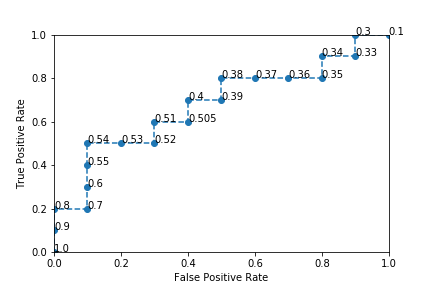
\includegraphics{ROC.png}


\end{document}